\chapter{Internet of Things}

\section{Inside IoT}
\subsection{Hardware components}
IoT devices contain \textbf{sensors}, \textbf{actuators}, or \textit{both}.
\begin{itemize}
   \item \textbf{Sensors} $\longrightarrow$ \textit{acquire data}\\
   Monitor Things and provide data about the Thing, like temperature, light intensity, or battery level.
   \item \textbf{Actuators} $\longrightarrow$ \textit{control/act on data}\\
   Control Things through hardware in the device;
   they represent the physical
   interface to the Thing that "make it go"
   \note{
      e.g. controls in a smart thermostat, dimmer switch in a smart light bulb, or motors in a robotic vacuum cleaner.
   }
\end{itemize}

All IoT devices have a way to process sensor data, store {--}if necessary{--} such data locally, and provide the computing power that makes the device
operate.
The data \textbf{processing component} of the IoT device coordinates data from multiple sensors or stores in flash memory.

\subsection{Firmware}
The \textbf{Firmware} is the onboard software that runs an IoT device sits between the
hardware and the outside world.

For simpler resource-constrained devices the firmware may be \textbf{embedded}.
More advanced devises instead nowdays have an entire \textbf{OS} as firmware, providing an
\textit{abstraction layer} between the hardware and other software on the device.

A popular choice is \href{https://busybox.net/}{\textbf{Busybox}}, which however is not a proper OS, but rather a small executable wrapping some key unix utilities, which for Desktop distributions are commonly found in the \texttt{coreutils} package.

\note{A whole OS is instead \href{https://github.com/contiki-ng/contiki-ng/wiki}{Contiki-NG}, an OS specifically designed for IoT constrained devices which, even if providing multitasking features and a -simple- GUI, needs only $\thicksim 10$KB RAM and its code footprint is about $\thicksim 100$KB}

\section{IoT Attacks}
\textbf{Security} is usually an \textit{\underline{afterthought}} in IoT because it is difficult to create a cheap, reliable, resource-constrained device that can connect to a wireless network, having \texttt{very little power consumption}.

\labelitemize{Attack Vectors}{
\begin{enumerate}
   \item \textbf{Weak Passwords}\\
   To simplify the device setup and use, the manufacturer offers typically weak login credentials
   \item \textbf{Lack of encryption}\\
   Many IoT devices do \textit{not} support encryption,
   to save battery and performance.
   \item \textbf{Backdoor}\\
   Is common practice for manufacturers to put "hidden" access mechanisms to simplify the support. 
   Once a backdoor becomes known, the manufacturer can either remove it, or make it more difficult to be accessed (or so they think \smiley)
   \item \textbf{Internet Exposure}\\
   Unlike a hardened server where you can control the firewall and how the host is accessed, most IoT
   devices have little or no security and accept most internet traffic, 
   making them susceptible to attack.
\end{enumerate}
}
\labelitemize{Countermeasures}{
   \begin{enumerate}
      \item Always \textbf{change} the \textit{default password}
      \item \textbf{Remove} devices with \textit{telnet backdoors}
      \begin{enumerate}
         \item To discover such devices you can use IoT device scanners that
         check with \href{https://www.shodan.io/}{\textbf{Shodan}}, an IoT search engine, to reveal if your devices
         are vulnerable based on the IP address of the scanning computer.
      \end{enumerate}
      \item \textbf{Never expose} a device directly to the internet
      \begin{enumerate}
         \item When you consider whether or not to expose a device to the
         internet by opening up your firewall, the right answer is almost
         \textbf{always no}.
      \end{enumerate}
      \item IoT device scanner can run a \textit{"deep scan"} to check for any open
      ports on your publicly exposed IP address assigned by your ISP.
      \begin{enumerate}
         \item \textbf{Port Scan} all your machines
      \end{enumerate}
   \end{enumerate}
}

\subsection{Shodan}
\href{https://www.shodan.io/}{\textbf{Shodan}} is a \textit{search engine} for finding specific devices, and
device types, that exist online.\\
The most popular searches are for things like webcam, linksys, cisco, netgear, SCADA, default passwords.

It uses a specialized scanner to \underline{scan the \textbf{entire Internet}} and parse the banners that are returned by various devices.
\note{
   Shodan can tell things like what web server {--}and
   version{--} is most popular, or how many anonymous FTP
   servers exist in a particular location, and what make and
   model the device may be.
}
You start by navigating to the main page, and then entering
into the search field, like you would any other search engine.

\begin{figure}[htbp]
   \centering
   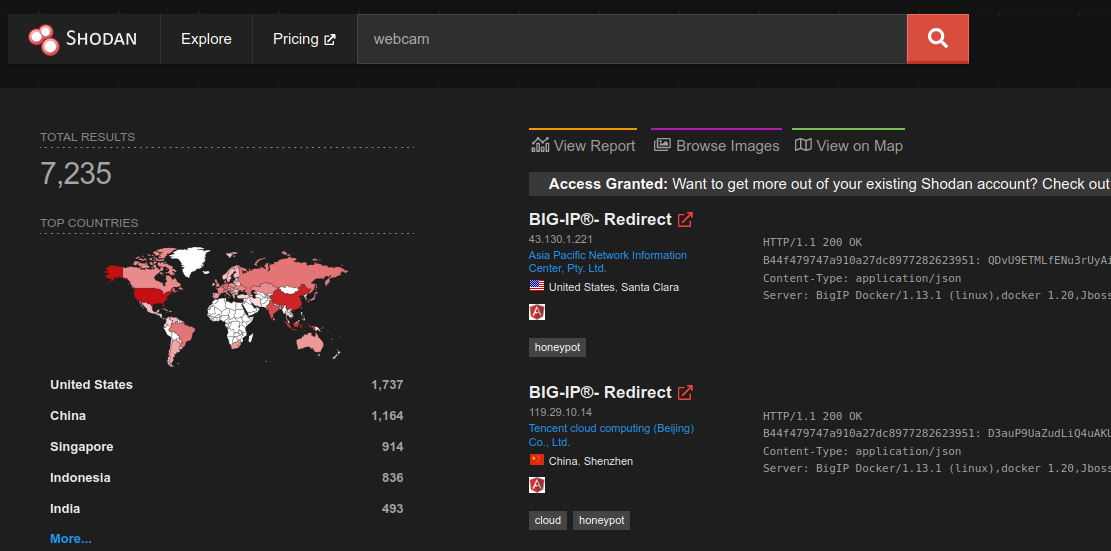
\includegraphics{images/shodan.png}
   \caption{Shodan search screenshot}
   \label{fig:shodan}
\end{figure}

\section{Device Classification}
IoT Nodes may be classified by performance or functionally
\labelitemize{Performance}{
\begin{enumerate}
   \item \textbf{Ultra-constrained} node\\
   RTOS or bare metal with 16K of RAM.
   Energy harvesting limits radio transmissions to conserve power.
   \item \textbf{Constrained} node\\
   RTOS with 32K-64K RAM.
   Most likely running on a battery and software optimised for battery life.
   Again minimizing radio transmission
   \item \textbf{Mainstream} node\\
   A feature rich RTOS with 128K RAM.
   More complex interaction with the context since there is room for more local operation, as opposed to sending all data upstream.
   \item \textbf{Gateway} node\\
   An advanced OS with 64MB RAM.
   A sophisticated node with advanced software and runs from main power.
   Multiple radios to support the local network.
\end{enumerate}
}

\labelitemize{Functional}{
\begin{enumerate}
   \item \textbf{Simple node}\\
   Not aware of the rest of the local network.
   It collects and
   reports information to the specified destination.
   Any of previous 1-3
   may be a simple node it depends upon interactions.
   \item \textbf{Smart node}\\
   fully aware of all other network nodes mainly via software
   that understands mesh networks, local topologies and authorised
   interactions between nodes in the same network.
   \item \textbf{Access node}\\
   the edge box to connect the local network to the Internet
   via whatever broadband link is appropriate for the application.
   It has
   multiple radios facing the local network.
   \item No restrictions on creating a node that is a smart node and acts as a
   gateway.
\end{enumerate}
}

\subsection{Architecture}
\textbf{Software productivity} requires 32 bit real time embedded processor to quickly
develop and release software to handle connectivity, security and IoT
applications while managing and controlling multiple sensors,
and since one node design may be used to
release products for multiple different markets,
software productivity is essential.

To optimize power consumption multiple processors may be required, each for a different task:
\begin{enumerate}
   \item handling radio stacks and connectivity, 
   \item managing the sensors and actuators
   \item running system and network stack
\end{enumerate}
\note{No need to wake up the main processor if the radio one may check for incoming messages}
    
For what concerns \textbf{memory},
most embedded systems include:
\begin{itemize}
   \item \textit{Flash} memory to store the program,
   \item \textit{SRAM} to store code and data
   \item \textit{ROM} to hold the basic system description
\end{itemize}

\section{Security in IoT}
Bruce Schneier thinks that
security even in a world where \textit{everything is connected}\footnote{(\st{connected car} $\longrightarrow$ \textit{computer with four wheels}, \st{connected refrigerator} $\longrightarrow$ \textit{computer that keeps things cold})} can be addressed as if there's \textit{"nothing new"} from standard ICT security processes.\\
Let's break down its point of view:

Schneier first consider some (common) issues concerning security, which are particularly relevant for the IoT world.
\begin{enumerate}
   \item Most software is poorly written
   \item Internet was never been designed to be secure
   \item Extensibility is a problem, because a computer is a universal Turing machine $\Longrightarrow$ \textit{\ul{if it is smart is vulnerable}}
   \item Complexity helps the attacker
   \item New vulnerabilities to interconnection
   \item Attacks always get faster, smarter and cheaper
\end{enumerate}


But what \textbf{changes} does IoT world introduce?
\begin{enumerate}
   \item \textbf{Automation}, \textbf{autonomy}, \textbf{physical} agents
   \item \textbf{Patching} becomes much more complex or impossible and
   patches should be available for all the life of the things not of
   the computer (you cannot replace the computer but the thing)
   \item The same vulnerability and the same attack work both in ICT
   and internet of things
   \item \textbf{Integrity} and \textbf{availability} are more important than
   confidentiality
   \note{leaking health records vs hacking a body device}
\end{enumerate}

Schneier is not completely wrong,
in fact most "old" vulnerabilities can strike also IoT devices, but there are three key points that are not negligible:
\begin{enumerate}
   \item the \textbf{physical} nature of IoT
   \item the \textbf{number} of devices
   \item the existence of \textbf{preloaded code}
\end{enumerate}
\nl

There are two kind of attacks regarding the security of an IoT device:
\begin{enumerate}
   \item \textit{Attack the device}\\
   Any smart device increases your system attack surface and its connection
   can result in new attacks, making the device an intermediate step aka \textit{"stepping stone"}
   \item \textit{Attack \textbf{from} the device}\\
   Any smart device can store some malware to attack your system, making attacks
   from the device possible even from simple smart nodes.
   \nl

   \item[]While most of security research has focused on the first issue, the \textit{second}
   one is becoming more and more critical.
\end{enumerate}

In general, note that IoT includes a huge number of devices with code that cannot be
easily accessed, tested or patched.\\
According to prof. \textbf{Baiardi}, \textbf{fuzzing} and \textbf{reverse engineering} will become more and more important to
analyze devices and preserve \textit{confidentiality} and \textit{integrity}.

\section{New perspective on Attacks}

The interaction of an IoT device with the physical world enables to
\textit{exploit physical properties} to attack an ICT system in new ways.
An interesting example are attacks against a voice interface using frequency that the interface can hear but the human user cannot hear, also known as \textbf{DolphinAttack}s.

\note{
   The attack is effective on popular speech recognition systems, e.g. Siri,
   Cortana and Alexa.
}

Countermeasures can either be hardware ---e.g. microphone enhancements to drop frequencies above 20Khz---, or software, ---e.g. classifying the signal to discover modulated voice---.

In late 2016 the \textit{Mirai botnet} launched $\sim 15k$ DDoS attacks, exploiting as nodes mainly embedded and IoT devices which exposed \texttt{SSH}/\texttt{Telnet} services;
the attack infrastructure attempted to login to such devices\footnote{IP cameras, DVRs, consumer routers} using a set of \underline{\textbf{46}} hardcoded passwords, some traceable to a vendor,
and then wait for commands from a C2 server.\\
A couple of interesting aspects of Mirai are the hardcoded list of IPs{--}composed of addresses belonging to \textit{US Postal Service}, \textit{Dept. of Defense}, \texttt{IANA}, \textit{HP} and \textit{General Electric}{--}which bots avoided when performing scans,
and its \textit{"territorial"} nature:
bots included scripts whose purpose was to eradicate other worms an trojans as well as prohibiting remote connections to the hijacked device.
\nl

A proposed taxonomy on attacks to IoT devices is based on how the attacker \textit{deviates} features from their "official" functionality,
resulting in 4 different categories:
\begin{enumerate}
   \item \textbf{Ignoring} the functionality\\
   The attacker \textit{ignores} any physical functionality of the IoT device, and considers it only as a standard connected computing device;
   Since most IoT devices are cheap and with minimal security protections,
   without the possibility to be upgraded or patched, they are the perfect target.\\
   These attacks are a serious threat but the least interesting ones because they
   are applicable to any networked device and are not unique to IoT devices.
   Nothing new so far, but huge $\#devices$
   \item \textbf{Reducing} the functionality\\
   The attacker tries to kill or limit the designed functionality of the IoT device, e.g. the TV/refrigerator stops working.
   Seems dull, but consider wide organizations or \textit{connected medical devices}:
   attacks on such devices may be fatal.\\
   An attacker may use \textbf{ransomware} to temporarily lock an
   \textit{expensive physical device} and demand a large payment to restore its
   functionality.
   \item \textbf{Misusing} the functionality\\
   These attacks use {--}rather than disabling{--} a functionality of the
   physical device, but in an incorrect or an unauthorized way,
   usually resulting in annoying pranks that do not violate integrity;
   e.g.the attacker turns on heaters in august.
   \item \textbf{Extending} the functionality\\
   Extending a functionality requires imagination and sophistication,
   but may result in harmful unexpected effects, like a Roomba opening the lock of a door.\\
   A concrete example exploited LED dimmering to transmit information.
\end{enumerate}

\section{Privacy Concerns}
When an IoT device is plugged into a home network it
will start collecting data and doing its job sending data "home" to the companies servers,
to provide the "smart" features.
It is not trivial to understand which data is \textbf{collected} who is \textbf{responsible} for such data.
Even if the timing of opening/closing the fridge seems useless,
the synergy and interconnection in the massive data going outside your home network,
may be used to infer important information,
e.g. the presence or absence of people in a house.

\section{IoT Best Practices}
On the $2^{nd}$ of November 2019,
the \textit{IoT Security Foundation} published a few guidelines regarding security for IoT systems.
Some of them are already discussed in the previous section, while in the following subsections we will address others.
\subsection{Physical Security}

Any interface used for administration  or testing should be (\textit{physically}) removed from the production device. 
The device should also make its circuitry physically \textit{inaccessible} to avoid \textbf{tampering},
and in general should be {--}along with its packaging{--} \textbf{tamper-evident}.  

\subsection{Secure Boot}
Firstly it is advised to always use the ROM-based \textbf{secure boot} function, generally implying a multistage bootloader initiated by {--}a minimal amount of{--} \textbf{read-only code} stored in a \textit{one-time programmable} memory.\\
Besides, a hardware-based tamper-resistant capability should be used to run the trusted authentication/cryptographic required for the boot process.

There are some attacks in booting called "\textit{Time of Check} to \textit{Time of Use}", which can be strongly limited by \textbf{validating} boot code \underline{immediately} before use at \textit{each boot stage}.

Lastly, any \textit{failure} in the boot sequence should \textbf{fail gracefully} in a safe and secure state.

\subsubsection{LogoFAIL}
A LogoFAIL attack consists three steps:
\begin{enumerate}
   \item The attacker prepares a malicious logo image and stores it into the ESP\footnote{EFI System Partition} or inside an unsigned section of a firmware update, and it restarts the device.\\
   \textit{No phyisical} access is required for this step.
   It can be performed by exploiting unpatched vulnerabilities in browsers, media-players, etc. or by gaining brief access to a device while it is unlocked.   
   \item During the boot process, vulnerable firmware will load the malicious logo from the ESP and parse it with a vulnerable image parser,
   thus the attacker can hijack the execution
   flow by exploiting a vulnerability in the parser itself.
   \item The attacker achieves arbitrary code execution during the DXE\footnote{Driver Execution Environment} phase, which means complete game-over for platform security.
\end{enumerate}

Note that malicious code \textit{\underline{never} reaches} the hard drive,
and that once the hijacked image is in place, reinstalling the OS or replacing the main drive, won't remove it,
ensuring that the device remains infected.

Attacks, such as LogoFAIL, starting from the firmware level can be leveraged to install
a bootkit and subvert any OS-level security mechanism, while
remaining completely \textit{undetectable} by security detection solutions.
Modern "below-the-OS" such as \textit{Secure Boot} are useles against this threat.\\
Note also that LogoFAIL, since it targets UEFI code and does not depend on a specific architecture, represents a \textbf{cross-silicon exploitation}.

\nl
LogoFAIL was discovered by researchers using \textbf{Fuzzing}:
\textit{"When the campaign finished, we were overwhelmed by the amount of crashes we
found, so much that triaging them manually was quite complicated"}
the researchers wrote. 
In all, they identified 24 unique root causes, 13 of which they believe were exploitable.

The results raised a vexing question:
\begin{center}
   \textit{If fuzzers identified so many exploitable vulnerabilities, why the developers of
   and the OEMs selling the devices hadn’t already used these tools and fixed
   the underlying bugs?}
\end{center}

\note{\textit{Fuzzing} is \underline{fundamental} according to prof. Baiardi}

\subsection{Secure OS}
The OS should include only the components (libraries, modules, packages, etc.) required to provide the functions of the IoT device.

The devices should be shipped with the latest stable OS release and should be configured with the most secure configuration available, e.g. disabling unused ports, protocols and services;
OS components should be kept updated throughout time.

The \textit{Least Privilege Principle} should be strictly applied to all directories and files, and the root file system should not be writeable by users and applications.

\subsection{Credential Management}
Every device should be uniquely \textbf{identifiable} by means of a factory-set \textit{tamper-resistant hardware identifier}.
\note{Recall \textit{ZeroTrust}, where authentication depends also on the device itself}

Only non-trivial \textbf{passwords} should be allowed, and they should be managed and stored properly using \textit{industry standard} \textbf{encryption} mechanisms.

Also \textbf{digital certificates} should be handled carefully, and a single certificate should not be used to identify more than one device.

\subsection{Secure Software Update}
Packages of new releases should be \textbf{encrypted} to hinder reverse engineering, and the
updated routine should always validate integrity and authenticity of a package update before the installation begins.

As for \textit{Secure Booting}, a \textbf{fail-safe} mechanism must be provided when performing updates.

\subsection{Side Channel Attack}
A \textbf{Side Channel} is an unintended/unanticipated capability to observe changes in the state
of a system, where system could be at the chip, board, application, device or network
level.

Side Channel Attacks deduce information based on these changes and then use that
information to exploit the system. 
For example monitoring variations in temperature,
timing of certain events, changes in power consumption, emissions of sound,
electromagnetic radiation at any frequency etc. can \textit{leak information} about the system
from which data may be inferred or deduced.

Monitoring of a system’s behavioural symptoms may be further augmented by using \textbf{Fault
Injection}, i.e. deliberately running a system under conditions outside those for which it was
designed, possibly allowing to establish side channels \textit{not} available under normal operation.